\documentclass[14pt]{extreport}
\usepackage{gost}
\usepackage{hyperref}
\usepackage{makecell}
\usepackage{ragged2e}
\justifying

\makeatletter
\@addtoreset{figure}{part}% Reset figure numbering at every part
\makeatother
\renewcommand{\thefigure}{\arabic{figure}}% Figure number is part.figure
\renewcommand{\thetable}{\arabic{table}}



%Тут можно вставить дополнительные пакеты

\begin{document}
\pagestyle{empty} %  выключаем нумерацию
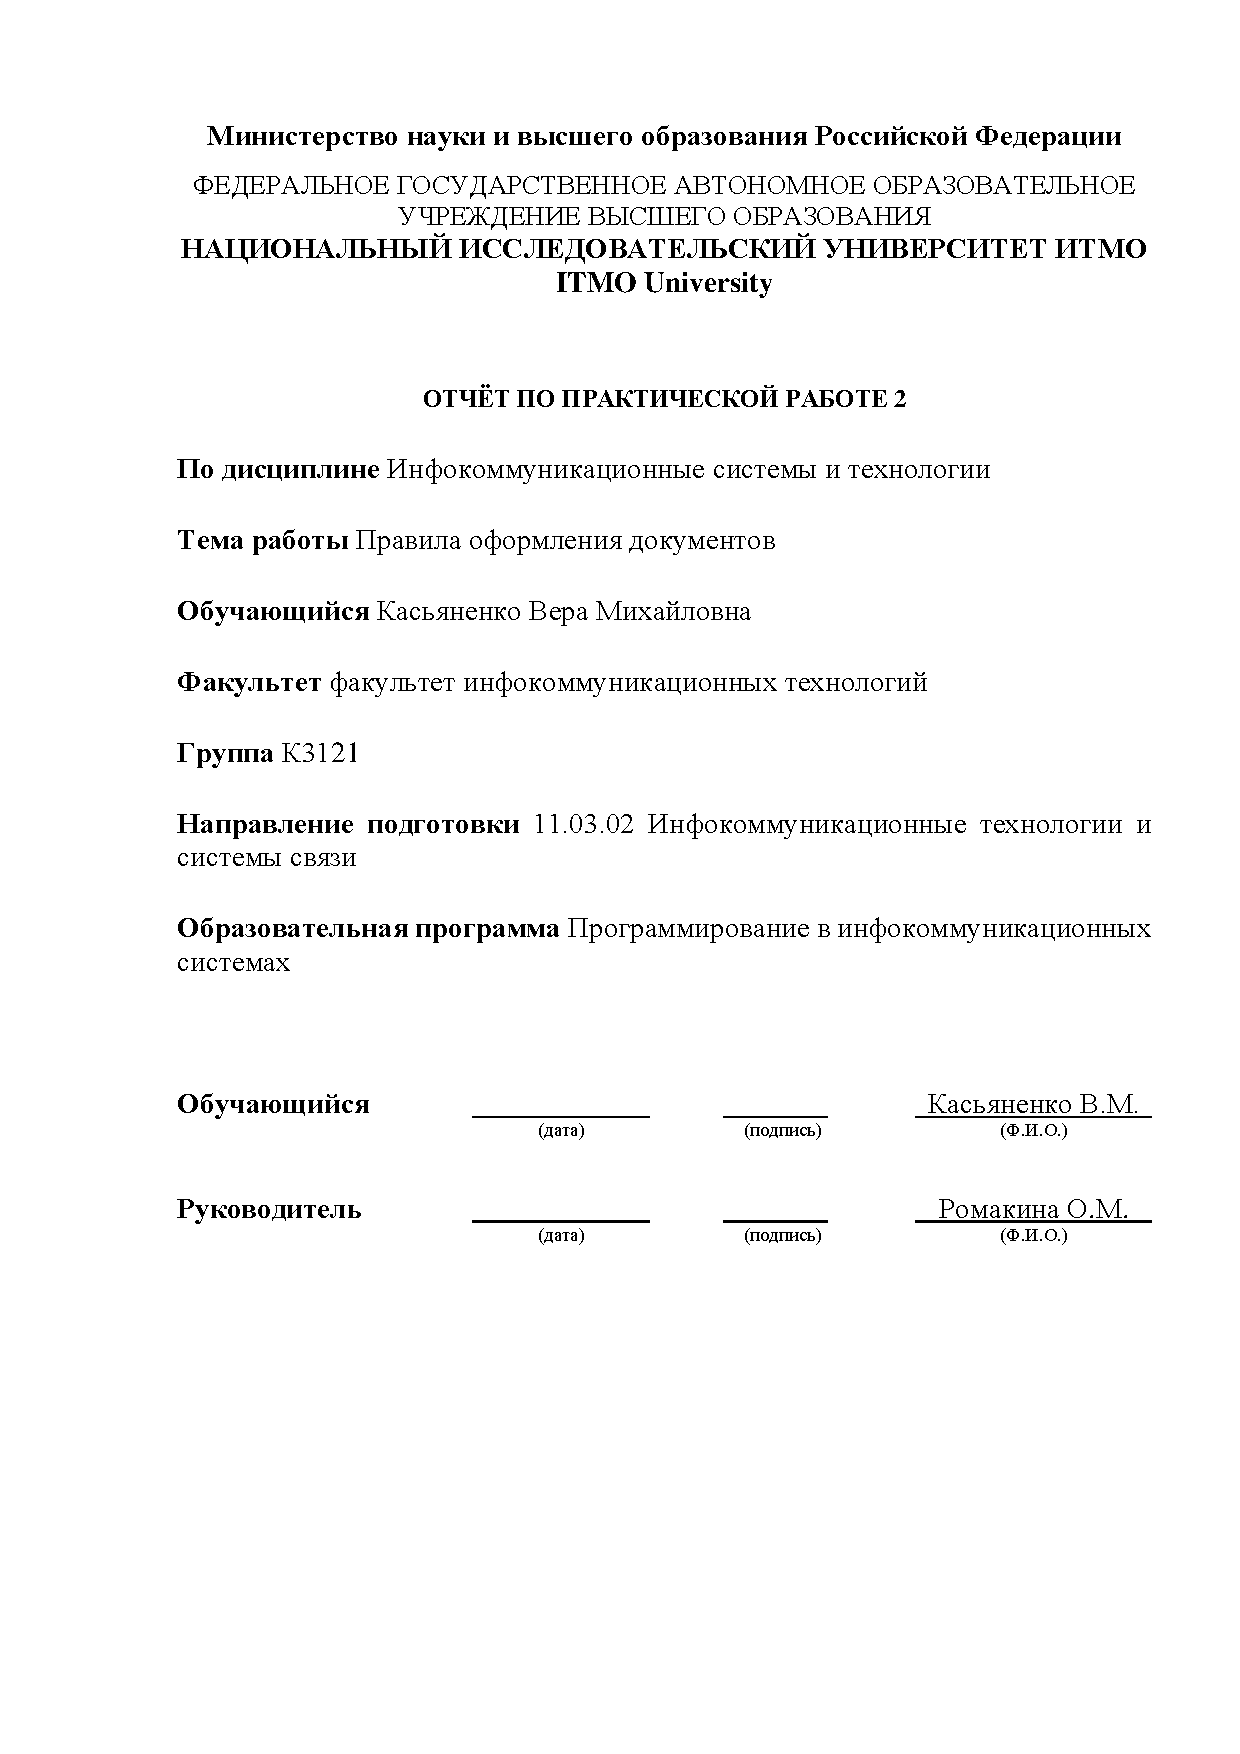
\includepdf[pages=-,pagecommand={}]{titulCourse.pdf}

\pagestyle{plain} % включаем нумерацию
\tableofcontents
 



\intro\label{intro}



Данный отчёт содержит пример оформления страницы из учебника по математическому анализу \cite{bib1} по ГОСТу, а также обзор рынка вакансий в сфере информационных технологий.


\chapter{МАТЕМАТИЧЕСКИЙ ТЕКСТ\label{chapter1}}
\section{Пример оформления математического текста}

Теоремы Лагранжа и Коши о конечном приращении. Следующее утверждение является одним из наиболее часто используемых и важных средств исследования числовых функций.

Теорема 1 (теорема Лагранжа о конечном приращении). Если функция 
 непрерывна на отрезке $f: [a,b] \rightarrow \mathbb{R}$ непрерывна на отрезке $[a,b]$ и дифференцируема в интервале $]a,b[$, то найдется точка $\xi\in]a,b[$,  такая, что
\begin{equation}\label{1} \tag{1}
f(b)-f(a)=f'(\xi)(b-a).
\end{equation}
 
$ \blacktriangleleft$ Для доказательства рассмотрим вспомогательную функцию
\[F(x)=f(x)-\frac{f(b)-f(a)}{b-a}(x-a),\]
которая, очевидно, непрерывна на отрезке $[a,b]$, дифференцируема в интервале $]a,b[$ и на его концах принимает равные значения: $F(a)=F(b)=f(a)$. Применяя к $F(x)$ теорему Ролля, найдем точку $\xi\in]a,b[$, в которой
\[F'(\xi)=f'(\xi)-\frac{f(b)-f(a)}{b-a}=0. \blacktriangleright\]

Замечания к теореме Лагранжа. 1° Геометрически теорема Лагранжа означает (рисунок~\ref{fig1}), что в некоторой точке $(\xi,f(\xi))$, где $\xi\in]a,b[$, касательная к графику функции будет параллельна хорде, соединяющей точки $(a,f(a)),$ $(b,f(b))$, ибо угловой коэффициент последней равен $\frac{f(b)-f(a)}{b-a}$.

2° Если $x$ интерпретировать как время, а $f(b)-f(a)$ – как величину перемещения за время $b-a$ частицы, движущейся вдоль прямой, то теорема Лагранжа означает, что скорость $f'(x)$ частицы в некоторый момент $\xi\in]a,b[$ такова, что если бы в течение всего промежутка времени $[a,b]$ частица двигалась с постоянной скоростью $f'(\xi)$, то она сместилась бы на ту же величину $f(b)-f(a)$. Величину $f'(\xi)$ естественно считать средней скоростью движения в промежутке $[a,b]$.

\begin{figure}[H]
\centerline{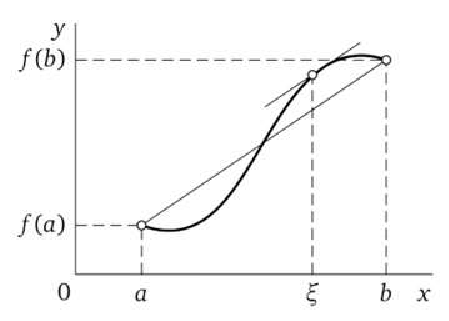
\includegraphics[width=0.5\linewidth]{Grafic}}
\caption{График}
\label{fig1} 
\end{figure}

 3° Отметим, однако, что при движении не по прямой средней скорости в смысле замечания 2° может не быть. Действительно, пусть, например, частица движется по окружности единичного радиуса с постоянной угловой скоростью $\omega=1$. Закон ее движения, как мы знаем, можно записать в виде
\[ r(t)=(\cos{t} ,\sin{t}). \]

Тогда
\[\dot{r}(t)=v(t)=(-\sin{t},\cos{t}) \]
и
\[\left|v \right|=\sqrt{\cos^2{t} + \sin^2{t}}=1.
\]

В моменты $t =0$ и $t =2\pi$ частица находится в одной и той же точке плоскости $r(0)=r(2\pi)=(1, 0)$, и равенство
\[ r(2\pi)- r(0) = v(\xi)(2\pi-0) \]
означало бы, что $v(\xi)=0$, но это невозможно.

Однако мы сознаем, что зависимость между перемещением за некоторый промежуток времени и скоростью движения все же имеется. Она состоит в том, что даже вся длина $L$ пройденного пути не может превышать максимальной по величине скорости, умноженной на время в пути. Сказанное можно записать в следующей более точной форме:
\[\left|r(b)- r(a)\right|\leq\underset{t\in]a,b[}{\sup}\left|\dot{r}(t)\right|\left|b - a\right|.\]

Как будет в свое время показано, это естественное неравенство действительно всегда справедливо. Его тоже называют теоремой Лагранжа о конечном приращении, а формулу (\ref {1}), справедливую только для числовых функций, часто называют теоремой Лагранжа о среднем значении (роль среднего в данном случае играет как величина $f'(\xi)$ скорости, так и точка $\xi$, лежащая между $a$ и $b$).

4° Теорема Лагранжа важна тем, что она связывает приращение функции на конечном отрезке с производной функции на этом отрезке. До сих пор мы не имели такой теоремы о конечном приращении и характеризовали только локальное (бесконечно малое) приращение функции через производную или дифференциал в фиксированной точке.


Следствие 1 (признак монотонности функции). Если в любой точке некоторого интервала производная функции неотрицательна (положительна), то функция не убывает (возрастает) на этом интервале.

$\blacktriangleleft$ Действительно, если $x_1, x_2$ — две точки нашего интервала и $x_1 < x_2$, то есть
$x_2 - x_1>0$, то по формуле (\ref {1})
\[f(x_2)- f(x_1) = f'(\xi)(x_2 - x_1), \text{где } x_1 < \xi < x_2,\]
и, таким образом, знак разности, стоящей в левой части равенства, совпадает со знаком $f'(\xi). \blacktriangleright$

Разумеется, аналогичное утверждение можно высказать о невозрастании (убывании) функции с неположительной (отрицательной) производной. 

Замечание. На основании теоремы об обратной функции и следствия 1, в частности, можно заключить, что если на каком-то промежутке $I$ числовая функция $f(x)$ имеет положительную или отрицательную производную, то функция $f$ непрерывна на $I$, монотонна на $I$, имеет обратную функцию $f^{-1}$, определенную на промежутке $I' = f(I)$ и дифференцируемую на нем.

Следствие 2 (критерий постоянства функции). Непрерывная на отрезке $[a, b]$ функция постоянна на нем тогда и только тогда, когда ее производная
равна нулю в любой точке отрезка $[a, b]$ (или хотя бы интервала $]a, b[$).

$\blacktriangleleft$ Интерес представляет только доказательство того факта, что если $f'(x)\equiv0$ на $]a, b[$, то для любых $x_1, x_2 \in[a, b]$ имеет место равенство $f (x_1)= f (x_2).$ Но это вытекает из теоремы Лагранжа, по которой
\[f (x_2)- f (x_1) = f'(\xi)(x_2 - x_1) = 0,\]
ибо $\xi$ лежит между $x_1$ и $x_2$, т. е. $\xi\in]a, b[$ и $f'(\xi)=0. \blacktriangleright$

Замечание. Отсюда, очевидно, можно сделать следующий (как мы увидим, очень важный для интегрального исчисления) вывод: если производные $F_1'(x), F_2'(x)$ двух функций $F_1(x), F_2(x)$ совпадают на некотором промежутке, т. е. $F_1'(x) \equiv F_2(x)$, то на этом промежутке разность $F_1(x) - F_2(x)$ есть постоянная функция.

Полезным обобщением теоремы Лагранжа, которое тоже основано на теореме Ролля, является следующее

Утверждение 2 (теорема Коши о конечном приращении). Пусть $x = x(t)$ и $y = y(t)$ — функции, непрерывные на отрезке $[\alpha, \beta]$ и дифференцируемые в интервале $]\alpha, \beta[$.

Тогда найдется точка $\tau\in]\alpha, \beta[$ такая, что
\[x'(\tau)( y(\beta)- y(\alpha)) = y'(\tau)(x(\beta)- x(\alpha)).\]

Если к тому же $x'(t) \neq 0$ при любом $t \in]\alpha, \beta[$, то $x(\alpha) \neq x(\beta)$ и справедливо
равенство
\[\frac{y(\beta)- y(\alpha)}{x(\beta)- x(\alpha)}=\frac{f'(\tau)}{x'(\tau)}.\]

$\blacktriangleleft$ Функция $F(t) = x(t)( y(\beta) - y(\alpha)) - y(t)(x(\beta) - x(\alpha))$ удовлетворяет условиям теоремы Ролля на отрезке $[\alpha, \beta]$, поэтому найдется точка $\tau\in]\alpha, \beta[$, в которой $F'(\tau) = 0$, что равносильно доказываемому равенству. Чтобы получить из него соотношение, остается заметить, что если $x'(t) \neq 0$ на $]\alpha, \beta[$, то по той же теореме Ролля $x(\alpha) \neq x(\beta). \blacktriangleright$

Замечания к теореме Коши. 1° Если пару функций $x(t), y(t)$ рассматривать как закон движения частицы, то $(x'(t), y'(t))$ есть вектор ее скорости в момент $t$, а $(x(\beta) - x(\alpha), y(\beta) - y(\alpha))$ есть вектор ее смещения за промежуток времени $[\alpha, \beta]$, и теорема утверждает, что в некоторый момент $\tau \in[\alpha, \beta]$ эти векторы коллинеарны. Однако этот факт, относящийся к движению в плоскости, является таким же приятным исключением, каким является теорема о средней скорости в случае движения по прямой. В самом деле, представьте себе частицу, равномерно поднимающуюся по винтовой линии. Ее скорость составляет постоянный ненулевой угол с вертикалью, в то время как вектор смещения может быть и вертикальным (один виток).

2° Формулу Лагранжа можно получить из формулы Коши, если в последней положить $x = x(t)=t, y(t)= y(x)= f (x), \alpha=a, \beta =b$.



\chapter{ОБЗОР РЫНКА ВАКАНСИЙ\label{chapter2}}

\section{Таблицы с мечтами}

В данном разделе рассматриваются вакансии 3 профессий, найденных на сервисе по подбору персонала \cite{bib2}: администратор баз данных (таблица~\ref{table1}), разработчик мобильных приложений для Android (таблица~\ref{table2}) и Backend разработчик (таблица~\ref{table3}). На основе полученных данных были составлены таблицы, отражающие названия вакансий, требования, предметы из учебного плана, которые помогут в получении знаний, а также преимущества и недостатки данных вакансий.

\begin{landscape}
Таблица 1 – Администратор баз данных
\begin{longtable}[H]{lp{1\linewidth}}
\caption{Администратор баз данных \label{table1}}


\centering

\begin{small}


    \begin{tabular}{|c|p{5,5cm}|p{6cm}|p{5cm}|p{5cm}|}
	\hline 
	\makecell{№ \\ п.п.} &	\makecell{Наименование,\\ должность, ссылка} &	\makecell{Требования} & 	\makecell{Дисциплины \\ из учебного \\плана} &	\makecell{Преимущества и \\недостатки}  \\ 
	\hline 
	1	& DBA/Администратор баз данных 
	
	(Senior/Team Lead)
	
(\url{https://goo.su/R8SD}) & •	Знание внутреннего устройства и ограничений СУБД PostgreSQL 

•	Опыт разработки архитектуры приложений, использующих БД больших объемов

 &	•	Проектирование и реализация баз данных
 
•	Компьютерные сети
 & + Гибкое время начала рабочего дня

+ Официальное трудоустройство 

- Далеко от метро\\
	\hline
	2 & Teamlead DBA PostgreSQL, MS SQL
	
(\url{https://goo.su/2tqbX})
& •	Опыт управления командой DBA 

•	Опыт администрирования ОС Windows, СУБД MS SQL, PostgreSQL, MongoDB
&
•	Администрирование сетей Windows

•	Коммуникации и командообразование
&+	Официальное трудоустройство 

+	Конкурентная заработная плата

-	Нужен опыт\\


	\hline
	3 & Руководитель отдела администрирования СУБД (PostgreSQL, MS SQL)
	
(\url{https://goo.su/avxun}) &
•	Опыт администрирования ОС Windows, Linux

•	Знание архитектуры MS SQL
&
•	Администрирование сетей Windows

•	Администрирование ОС Linux
&
+	Корпоративное обучение и электронная библиотека

-	Полная занятость
\\
	\hline


    \end{tabular}
\end{small}
\end{longtable}

\addtocounter{table}{-1}
\newpage
Продолжение таблицы 1
\begin{longtable}[H]{lp{1\linewidth}}
\caption{Продолжение таблицы 1}



\centering
\begin{small}


    \begin{tabular}{|c|p{5,5cm}|p{6cm}|p{5cm}|p{5cm}|}
	\hline 
	\makecell{№ \\ п.п.} &	\makecell{Наименование,\\ должность, ссылка} &	\makecell{Требования} & 	\makecell{Дисциплины \\ из учебного \\плана} &	\makecell{Преимущества и \\недостатки}  \\ 
	\hline 
4 & Разработчик БД MySQL (Senior)

(\url{https://goo.su/Ex9c}) 
 & •	Написание хранимых процедур на SQL с максимальным набором алгоритмических возможностей 

•	Построение отказоустойчивых БД системы на базе MySQL или аналогичных реляционных БД &
•	Проектирование и реализация баз данных &
+	Транспортная доступностью

+	Гибкое начало рабочего дня

-	Полная занятость\\
\hline
5 & Администратор баз данных (PostgreSQL) 

(\url{https://goo.su/7OAzx}) & •	Уверенные знания одной или нескольких СУБД: Oracle, MSSQL, PostgreSQL

•	Опыт резервирования и восстановления работоспособности БД & •	Проектирование и реализация баз данных & 
+	Удаленный формат работы

-	Нужен опыт работы\\

	\hline

    \end{tabular}
    \end{small}
\end{longtable}

Выводы из таблицы~\ref{table1}: относительно мало вакансий, однако довольно большая заработная плата и хорошие условия труда, а также в учебном плане есть много предметов, которые помогут овладеть нужными знаниями.




\newpage
Таблица 2 – Разработка приложений для Android
\begin{longtable}[H]{lp{1\linewidth}}

\caption{Разработка приложений для  \label{table2}}


\centering

\begin{small}


    \begin{tabular}{|c|p{5,5cm}|p{6cm}|p{5cm}|p{5cm}|}
	\hline 
	\makecell{№ \\ п.п.} &	\makecell{Наименование,\\ должность, ссылка} &	\makecell{Требования} & 	\makecell{Дисциплины \\ из учебного \\плана} &	\makecell{Преимущества и \\недостатки}  \\ 
	\hline 
	1	& Senior Android разработчик
	
(\url{https://goo.su/SPSpnCF}) &
•	Большой практический опыт разработки приложений под Андроид

•	Знание Java, Android, Java SE, ООП, Kotlin &
•	Прикладное программирование

•	Разработка приложений на Java &
+	Удаленная работа


+	Почасовая оплата

-	Неофициальное трудоустройство \\

	\hline
	2	& C++developer (Senior)
	
(\url{https://goo.su/bA7lqc}) &
•	Опыт разработки на С++11/17/20

•	Опыт разработки на Java под Android 

•	Знание английского языка на уровне чтения технической документации &
•	Программирование на C++

•	Прикладное программирование

•	Разработка приложений на Java &
+	Официальное трудоустройство 

+	Возможность выбора оборудования для работы

-	Знание английского\\
	\hline 
	3	& Старший Android разработчик 
	
(\url{https://goo.su/pcY9UpZ}) &
•	Отличные знания Kotlin/Java, Android SDK

•	Знание сетевых протоколов &
•	Компьютерные сети

•	Разработка приложений на Java &
+	Оформление по ТК РФ

+	Гибкое начало рабочего дня 

-	Нужен опыт \\


	\hline


    \end{tabular}
    \end{small}
\end{longtable}




\addtocounter{table}{-1}
\newpage
Продолжение таблицы 2
\begin{longtable}[H]{lp{1\linewidth}}
\caption{Продолжение таблицы 2}

\centering

\begin{small}


    \begin{tabular}{|c|p{5,5cm}|p{6cm}|p{5cm}|p{5cm}|}
	\hline 
	\makecell{№ \\ п.п.} &	\makecell{Наименование,\\ должность, ссылка} &	\makecell{Требования} & 	\makecell{Дисциплины \\ из учебного \\плана} &	\makecell{Преимущества и \\недостатки}  \\ 
	\hline 
	4	& Senior Android Developer
	
(\url{https://goo.su/w72dZi}) &
•	Знание Kotlin 
•	Опыт работы с Git, Dagger 2, RxJava
& 
•	Прикладное программирование &
+	Гибкий график

+	Возможность работать в офисе или дома

-	Полная занятость \\

	\hline
5	& Senior android-разработчик 

(\url{https://goo.su/6xssM}) &
•	Знание Java, Kotlin, ООП

•	Понимание и опыт работы с Git

•	Опыт работы с ресиверами, SQLite, структурами данных &
•	Разработка приложений на Java

•	Информатика &
+	Участие в крупных и интересных проектах

+	Комфортный современный офис

-	Полная занятость \\


	\hline 


    \end{tabular}
    \end{small}
\end{longtable}
Выводы из таблицы~\ref{table2}: много интересных разнообразных задач, которые ставятся перед разработчиком, огромное количество вакансий, учебный план не может дать все необходимые знания, многому предстоит научиться самому.







\newpage
Таблица 3 – Backend разработка
\begin{longtable}[H]{lp{1\linewidth}}
\caption{Backend разработка \label{table3}}


\centering

\begin{small}


    \begin{tabular}{|c|p{5,5cm}|p{6cm}|p{5cm}|p{5cm}|}
	\hline 
	\makecell{№ \\ п.п.} &	\makecell{Наименование,\\ должность, ссылка} &	\makecell{Требования} & 	\makecell{Дисциплины \\ из учебного \\плана} &	\makecell{Преимущества и \\недостатки}  \\ 
	\hline 
	1	& Senior Backend Developer 
	
(\url{https://goo.su/JiLMD6G}) &
•	Опыт работы с базами

•	Английский язык на уровне, достаточном для переписки и общения в чате &
•	Проектирование и реализация баз данных

•	Иностранный язык &
+	Возможностью работать удаленно

+	Премиальная система

-	Знание английского \\


	\hline
	2	& Senior Backend Developer
	
(\url{https://goo.su/r4Wuh}) &
•	Понимание архитектуры и принципов разработки web-приложений

•	Разработка кода backend части проекта &
•	Web-программирование &
+	Полностью удаленная работа

-	Нужен опыт
\\

	\hline 
	3	& Senior Java Backend Developer
	
(\url{https://goo.su/xzGWo5R}) 	&
•	Хорошее знание и опыт программирования на Java и/или Kotlin

•	Умение работать в команде &
•	Разработка приложений на Java

•	Коммуникации и командообразование &
+	Работа в аккредитованной IT – компании.

+	Бесплатные завтраки и ужины, компенсация обедов

-	Полный рабочий день \\


	\hline


    \end{tabular}
    \end{small}
\end{longtable}

\newpage
Продолжение таблицы 3
\begin{longtable}[H]{lp{1\linewidth}}
\caption{Продолжение таблицы 3}

\centering

\begin{small}


    \begin{tabular}{|c|p{5,5cm}|p{6cm}|p{5cm}|p{5cm}|}
	\hline 
	\makecell{№ \\ п.п.} &	\makecell{Наименование,\\ должность, ссылка} &	\makecell{Требования} & 	\makecell{Дисциплины \\ из учебного \\плана} &	\makecell{Преимущества и \\недостатки}  \\ 
	\hline 
	4	& Senior/TechLead Backend разработчик
	
(\url{https://goo.su/EY07u0}) &
•	Знание JavaScript

•	Опыт работы с Unix/Linux &
•	Информатика

•	Web-программирование &
+	Удаленный формат работы

-	Нужен опыт работы
\\



	\hline
	5	& Senior .Net Backend Developer
	
(\url{https://goo.su/ombjxS}) &
•	Опыт разработки на C\# 

•	Опыт работы с Docker

•	Отличное понимание архитектурных паттернов 

•	Опыт работы с брокером сообщений &
•	Алгоритмы и структуры данных

•	Прикладное программирование & 
+	3 дня в офисе, 2 дня удаленно
 
+	Производительная техника для комфортной работы

-	Нужен опыт
\\

	\hline 


    \end{tabular}
    \end{small}
\end{longtable}

Выводы из таблицы~\ref{table3}: достаточно много вакансий с удаленным форматом, требуется относительно мало знаний, большинство из которых может обеспечить учебный план, однако не самые интересные задачи. 
\end{landscape}



\conclusions

Был составлен отчет, в котором приведен пример математического текста, оформленного по ГОСТу, а также произведен обзор рынка вакансий, на основе которого были составлены некоторые выводы.



\newpage
\begin{thebibliography}{99}
\bibitem{bib1} Зорич, В. А. Математический анализ. Часть I. — Изд. 10-е, испр. — М.: МЦНМО, 2019. — XII+564 с.

\bibitem{bib2} HeadHunter: официальный сайт. – URL: \url{http://spb.hh.ru} (Дата обращения 07.09.2022).
\end{thebibliography}







\end{document}
